\documentclass{article}
\usepackage[utf8]{inputenc}
\usepackage{amsmath}
\usepackage{amssymb}
\usepackage[margin= 1.25in]{geometry}
\usepackage{mathtools}
\usepackage{booktabs}
\usepackage{multirow}
\usepackage[framed]{matlab-prettifier}
\usepackage{graphicx}
\usepackage{subcaption}
\usepackage[shortlabels]{enumitem}
\usepackage{cite}
\usepackage{grffile}

\graphicspath{{plots/desc-stats/}{plots/}{plots/corr-mats/}}

\begin{document}
\title{Predicting Baseball Game Outcomes:\\
Using Weather Data and Recursive Logistic Regression}
\author{Brendan Whitney}
\date{\today}
\maketitle

\begin{abstract}
    This paper attempts to build a regression model to predict the winner of 
    baseball games for the 2018 MLB season.
    The regression model is built from two disjoint datasets:
    baseball statistics from baseball-reference.com
    and weather data from the Global Historical Climatology Network.
    The text presents initial results from an exploration of the data combined 
    to create the full dataset.
    Then the regression model is created and analyzed using recursive models
    that are trained on the previous games before predicting the games for 
    each day of the season.
    The model had a predictive power of 55.77\%,
    which is more predictive than coin flips.
    However,
    the model did not have more predictive power than just simply choosing
    the team with the highest win percentange or Pythagorean score.
\end{abstract}

\section{Introduction}
Predicting the outcome of sports games is a very difficult problem,
and has been studied for a while now.
There are many factors that go into the outcome of a game,
and what appears to be a lot of luck involved as well.
Additionally,
many factors that affect the outcome of a game are often not reflected in the
pure statistics of the teams entering the contest.
Considering just statistics of the two teams does not include other potentially
important information,
such as injuries to important players,
or the atmosphere of the team \cite{Boulier}.
That extraneous information has long been believed to play a role in the
results of contests.
This manifests itself in what we would consider to be luck,
and plays into the notion that everytime two teams play each other "its
anyones game".
Perhaps what we currently percieve as luck in sports games is instead simply
not having the vital data required to correctly predict outcomes. \par

Building off of work done by Boulier and Stekler regarding predicting the
outcomes of National Football League games \cite{Boulier},
I attempt to predict the outcome of games in the MLB.
Boulier and Stekler utilize the New York Times power ranking algorithm to 
test whether the power ranking was a useful measure for predicting the outcome
of games.
They introduced a home-field model as their baseline
-- this model simply picked the home team as the winner --
and tested it against the power rankings,
the betting predictions,
and the sports editors predictions.
From the initial predictions,
the betting predictions were the most accurate,
followed by choosing the home team,
then the power rankings,
and finally the sports editors were the worst predictors out of the four.
However,
they also showed that all four results of the rankings,
were significantly different from a binomial distribution with p=0.50.
We see that there are predictive powers in each case,
but even the betting predictions were only able to correctly predict the
winner about 66\% of the time.
It seems there is potentially significant room for improvement. \par

Other literature on the topic of game prediction for baseball,
introduced the idea of the Pythagorean Formula
for predicting end of season win percentage for a given team.
The Pythagorean Formula is defined as:
\[
    \cfrac{RS_{obs}^\gamma}
    {RS_{obs}^\gamma + RA_{obs}^\gamma}
\]
Where $RS_{obs}$ represents the number of observed runs scored for a team,
and $RA_{obs}$ represents the number of observed runs allowed for a team.
$\gamma$ is an exponent that is constant for all the teams in the league.
Originally proposed by statistician and baseball writer Bill James,
the Pythagorean Formula was given statistical proof by Steven Miller in 2007.
Miller determined from a Weibull distribution built from the Pythagorean 
Formula that $\gamma=1.79$ was the best fit for the American League teams in
2014 \cite{Miller}.
The theoretical model also shows that the runs scored and allowed per game
are statistically independent events,
which makes them useful for modeling the winner of the games.
Finally,
Miller concludes that since the calculation of $\gamma$ results from 
an analysis of the distribution of scores of individual baseball games,
then it can be used to predict future success.
Therefore,
the Pythagorean Formula will be very important for the task of prediction
for the 2018 season.\par

An article written by Cesar Soto-Valero regarding the use of data
mining techniques to enhance predictive techniques lent many good ideas 
regarding the construction of the data for improved predictive performance
\cite{Cesar}.
Soto-Valero utilizes cumulative statistics to represent the knowledge of 
a season entering a particular game.
This method of accumulating information as the season progresses will be
instrumental to the success of the recursive logit regression,
similar to the method used by Boulier and Stekler.
Additionally,
Soto-Valero uses subset generation to determine the best collection of features
for prediciton.
Therefore,
there is justification for the use of a Random Forest regression to determine
feature importance for the model.


\section{Data}
The baseball data for my project is scraped from baseball-reference.com.
The data comes from the schedule pages for each of the teams,
and includes various basic stats regarding each game.
The stats included are the location of the game (derived), the opponent,
the runs scored, the runs allowed, the resulting record, and the resulting
streak of the team.
From the scraped data,
the game data was shifted one game forward,
and the data for runs were cumulatively summed.
Therefore,
the data represents the statistics available at the beginning of each game,
which ensures that the predictive model is not given information regarding
the game it is attempting to predict.
Once the schedules were processed,
games were created by matching opponents and dates.
The games used the incoming cumulative runs scored,
cumulative runs allowed,
current records,
and current streaks of both teams.
From these statistics,
Pythagorean scores and the win percentages of each team were calculated.
For the Pythagorean score an exponent of 1.79 was used as per the Miller paper.
The target variable of interest is whether the home team won the game.\par

Figure~\ref{Fig:GPD} indicates the distribution of the number of games played
per day over the course of the season.
\begin{figure}[ht]
    \centering
    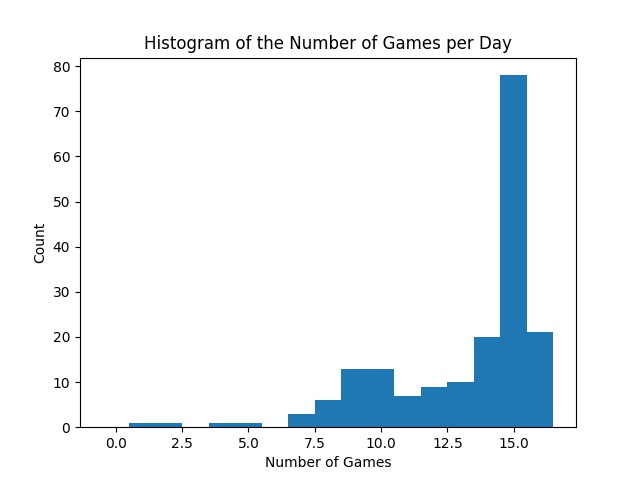
\includegraphics[width=.8\textwidth]{num-games-hist.jpg}
    \caption{Figure~\label{Fig:GPD} represents the distribution of number of 
    games played per day.}
\end{figure}
The number of games per day must be at least 1 and
technically has a max value of 30 if every team played a double header.
However,
from the above histogram,
we see the max number of games played was 16,
which ocurred 20 times.
The values are heavily skewed towards the upper end of the range of games,
which makes sense given the fact that the MLB would want to as many games
as possible to be played every day.


To supplement the baseball data in hopes of improved accuracy,
historical weather data was added to the games.
Baseball is a sport that is played in open air stadiums,
and the season is long enough that players experience colder temperatures
on either end of the season and endure the hottest months during the middle of
the season.
It is important to note that games are not played in heavy rain.
The weather data comes from the Global Historical Climatology Network (GHCN) 
Database stored on Google's Big Data Query (BDQ).
GHCN records the maximum temperature (TMAX),
minimum temperature (TMIN),
precipitation (PRCP),
snowfall (SNOW),
and snow depth (SNWD) as the core elements of recording.
Other important aspects of the weather are unfortunately not as reliably
recorded,
thus barring them from inclusion.
Additionally,
SNOW and SNWD were ignored from the dataset because games are either cancelled
due to excessive snow,
or the snow is removed from the playing surface before a game is played.
Therefore,
the SNWD and SNOW values do not accurately reflect the conditions while the
game is being played. \par

Weather for the entire season was pulled from the closest active weather
stations to each ballpark.
The distance from each ballpark was measured by the Haversine equation on 
the latitudes and longitudes of the stadiums and stations.
The 2018 season was played from March, 29th to October, 1st.
All stadiums were treated as open air stadiums despite the fact that
6 stadiums have retractable roofs,
and one stadium,
Tropicana Field -- home of the Tampa Bay Rays,
has a fixed roof. 
Figure~\ref{Fig:Weather} shows the data gather for Fenway Park,
home of the Boston Red Sox,
as an example for how the weather data was used.
\begin{figure}[ht]
    \centering
    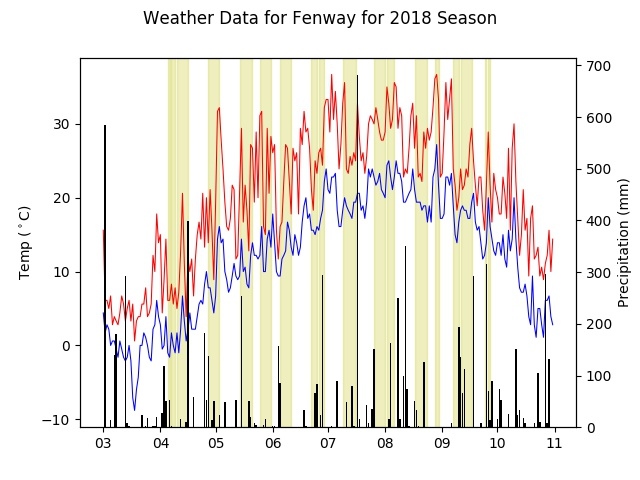
\includegraphics[width=.8\textwidth]{weather-example.jpg}
    \caption{Figure~\label{Fig:Weather} represents the daily weather data for
    Fenway Park.  The red line indicates maximum temperature and the blue
    line indicates minimum temperature both measured using the left y-axis.
    The black bars represent the precipitation measured using the right y-axis.
    The yellow bands indicate the dates where Red Sox played games,
    and represent the days that the weather data was incorporated into the
    baseball data.}
\end{figure}
Despite having weather data from March 1st to October 31st,
a small portion of that data was actually used by the regression model.
The portion used is indicated by the yellow vertical bands. \par

Both datasets were constructed completely by hand,
and represent a significant amount of time and  energy spent on this project.
Locally,
all stages of dataset construction and transformation are stored in csv files,
in their respective directories,
which indicate what transformation was applied to the data.
As an example,
the csv files found in the series folder contain game information for each
series during the season.
Those files are saved in the format \%HomeTeam-\%AwayTeam-\%Date.csv,
where \%Date indicates the starting date for the series.
The final dataset used for the intial models and the full season regression
is named 2018-combined.csv,
and is located at the top level of the data/ directory.
Use of Big Query for weather data limited the scope of this project to just
the 2018 season,
due to the time-consuming nature of pulling the records one station at a time.

\section{Methods}
Once the season was aggregated,
the initial exploration checked the predictive power of the important variables
home-field advantage,
win percentage,
and Pythagorean score introduced from the research.
The results of this initial exploration are found in the results section.
Then,
the correlation between each variable was calculated prior to the regression
to check the validity of using certain variables for prediction.
Logistic regression does not perform well with variables expressing 
multicollinearity.
Figure~\ref{Fig:Corr}(a) shows the correlation matrix for each variable for the
complete 2018 season.
The correlation matrix for the season indicates high correlation between all
of the non-calculated 
(ie. not win percentage or Pythagorean score) baseball statistics.
This high correlation can be explained by two factors,
the first being that all of the statistics increase monotonically as the 
season progresses.
Secondly,
the teams play in series of games,
which means one team plays another team multiple games in a row.
Therfore,
however many runs one team scores is exactly the number of runs the other team
has allowed for most of the season.
Variability is introduced when teams aren't playing each other,
but playing in series directly increases the correlation between the 
home and away variables.\par

To address the correlation issues created by series play,
one game was sampled from each series to create artificial seasons for
regression.
1000 artificial seasons were generated for analysis.
The sampled seasons consisted of 774 games played,
which remained enough games to justify using logistic regression for 
prediction.
Figure~\ref{Fig:Corr} shows a direct comparison between the correlation matrix
for the complete 2018 season,
and the sampled season 000.
3(b) shows a correlation matrix for the first sampled 
season.
\begin{figure}
    \centering
    \begin{subfigure}{0.75\textwidth}
         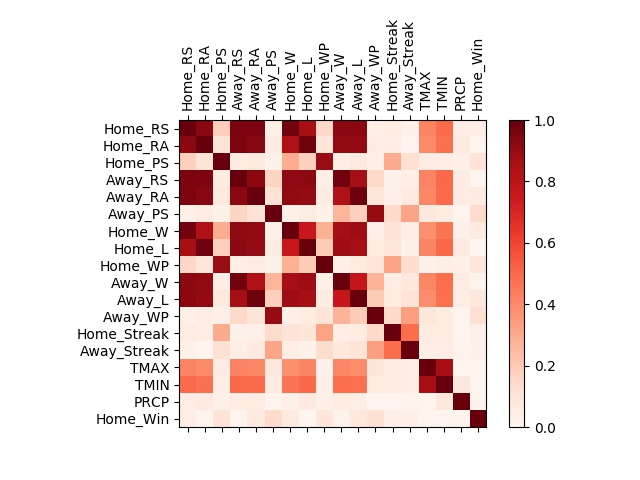
\includegraphics[width=\textwidth]{full-season/combined-stats-corr-mat.jpg}
         \caption{Correlation Matrix for the full season}
         \label{Fig:SeasonCorr}
    \end{subfigure}
    
    \begin{subfigure}{0.75\textwidth}
         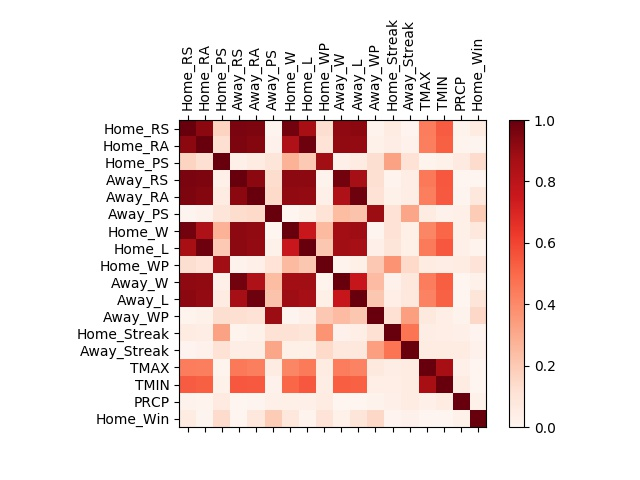
\includegraphics[width=\textwidth]{sampled-season/combined-stats-corr-mat.jpg}
         \caption{Correlation Matrix for the sampled season}
         \label{Fig:SampleCorr}
    \end{subfigure}

    \caption{Figure~\label{Fig:Corr} shows the correlation matrices for each 
    variable for the complete 2018 season and the sampled season 000.
    White spaces indicate little to no 
    correlation, and dark red spaces indicate nearly perfect positive or 
    negative correlation.}
\end{figure}
omparison between the correlation matrix for the complete season and sampled
season 000,
indicates no difference in the multicollinearity of the data.
Therefore,
simply passing the variables as-is to the logistic regressor was not possible.
\par

To handle the high correlations between many of the variables,
a Random-Forest Regressor (RFR) was used for feature extraction on the complete
2018 season.
To simulate the progression of the season,
the RFR was trained every day of the season on all of the games played up
until that point.
After training the RFR,
the feature importance scores were recorded.
From the RFR,
the six most important variables were chosen, where importance was
averaged over the entire season.
Table~\ref{Tab:Importance}
\begin{table}[ht]
    \centering
    \begin{tabular}{l | c c c c c c}
        Feature &  Away\_PS & TMAX & Home\_PS & TMIN & HOME\_WP & AWAY\_WP \\
        \midrule
        Importance Score & 0.111 & 0.101 & 0.098 & 0.089 & 0.076 & 0.075 \\
    \end{tabular}
    \caption{Table~\label{Tab:Importance} indicates the 6 most important
features ranked from most to least important.}
\end{table}
Figure~\ref{Fig:RFR} displays the feature importance scores as the season
progresses.
\begin{figure}[ht]
    \centering
    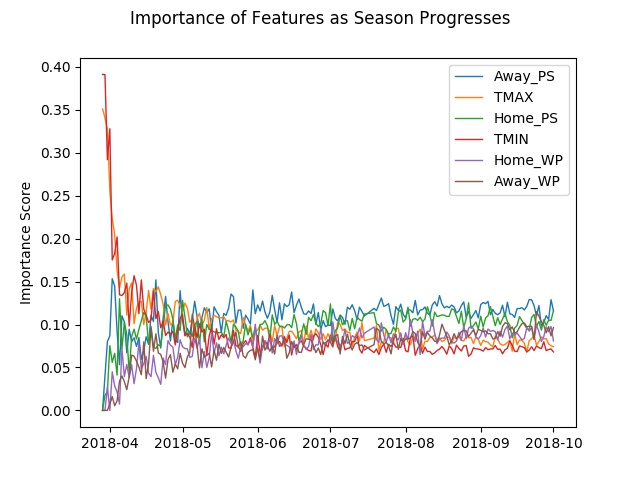
\includegraphics[width=.8\textwidth]{feature-importance.jpg}
    \caption{Figure~\label{Fig:RFR} shows the importance of the 6 most 
    important features as the season progresses from March 29th to October 1st.}
\end{figure}
As the figure indicates,
TMAX and TMIN are very important at the beginning of the season before the
win percentages and Pythagorean scores settle down with the accumulation of
data.
However,
the importance of TMAX and TMIN reduces very quickly,
and after July they are the two least important of the six variables used for 
logistic regression. \par

Following RFR,
a logistic regressor was constructed for each day of the season training on
the data from dates before the day,
and predicting the outcomes of that day.
This mechanism necessitated not predicting the first day of the season due to
the lack of prior data.
The beginning of the season was considered a clean slate,
and no information carried over from the end of the previous season.
These logistic regressors were calculated for the full 2018 season,
and for each of the simulated seasons.
The results from the simulated seasons were compiled and analyzed as a single
distribution of accuracy.

\section{Results}
\subsection{Initial Models and Statistics}
For initial analysis of the baseball data,
home-field advantage was calculated,
as well as using win percentage and Pythagorean Score as predictors of the
winner.
For the home-field advantage calculation,
the accuracy was derived from the sum of wins by home team divided by the 
total number of games.
The accuracy of predicting the home team as the winner was recorded for each 
day of the season with games.
Figure~\ref{Fig:Home-Field} indicates the daily accuracy of always picking the 
home team to win the game.
\begin{figure}[ht]
    \centering
    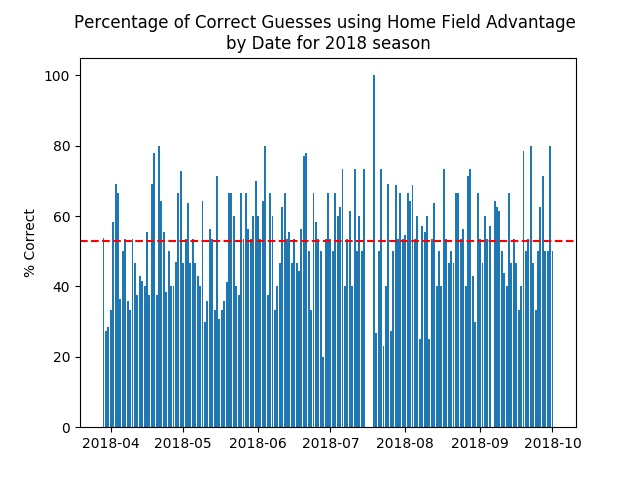
\includegraphics[width=.8\textwidth]{home-correctness.jpg}
    \caption{Figure~\label{Fig:Home-Field} represents the daily accuracy of 
    predicting the home team as the winner.  The red line indicates the season
average of 52.86\%}
\end{figure}
For 2018,
1283 home teams won in 2431 games played,
which means the home team won 52.87\% of the games.
When the proportion of home team wins were broken down by day,
the standard deviation per day was 14.45\%.\par

To use the win percentage as an indicator of the victor of each game,
the team with the highest win percentage was chosen as the victor.
Win percentage is calculated from the wins and losses of each team according to
this simple formula:
\[
    WP
    =
    \cfrac{W}{W+L}
\]
If two teams had the same win percentage,
the home team was predicted as the winner because of the slight advantage home
teams have of winning.
Figure~\ref{Fig:WP} represents the daily accuracy of predicting winners from 
their win percentage.
\begin{figure}[ht]
    \centering
    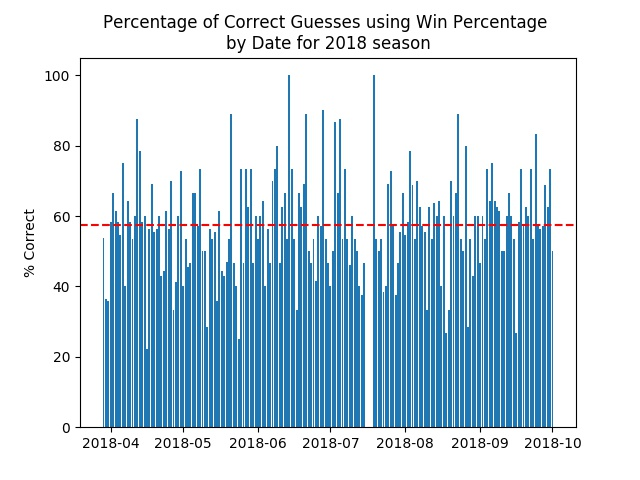
\includegraphics[width=.8\textwidth]{wp-correctness.jpg}
    \caption{Figure \label{Fig:WP} represents the daily accuracy of using win
    percentage as a predictor.  The red line indicates the season
average of 57.47\%}
\end{figure}
Win percentage was a better predictor of game outcomes than home-field advantage
alone.
Win percentage predicted the correct outcome of the game 57.47\% of the time
with a standard deviation of 14.17\%.
Therefore,
win percentage was not only more frequently correct,
but the variation in the predictions was reduced as well.
Both are improvements compared to the home-field results when considering the
desired result of accurate game predictions.\par

The Pythagorean score was tested as an indicator of predictive success.
Using the formula described in the introduction,
Pythagorean score was utilized similarly to win percentage.
If the scores were the same,
the home team was chosen as the winner.
Otherwise,
the team with the higher Pythagorean score was chosen as the victor for the
game.
Figure~\ref{Fig:PS} represents the daily accuracy of predicting winners from 
their win percentage.
\begin{figure}[ht]
    \centering
    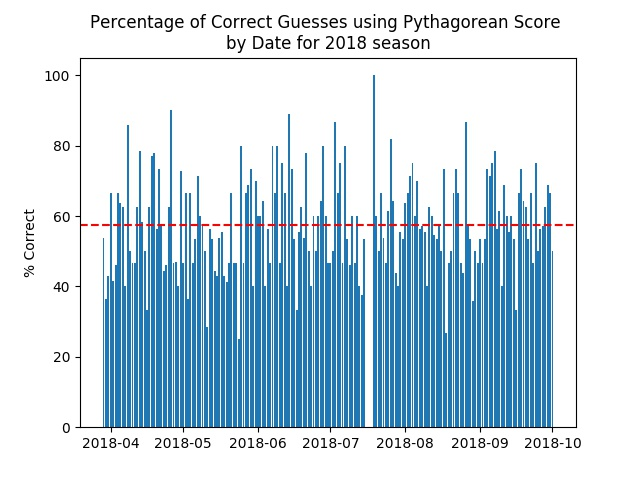
\includegraphics[width=.8\textwidth]{ps-correctness.jpg}
    \caption{Figure \label{Fig:PS} represents the daily accuracy of using
    Pythagorean score as a predictor.  The red line indicates the season
average of 57.56\%}
\end{figure}
The Pythagorean score slightly improved upon win percentage as a predictor.
Both the accuracy,
57.56\% compared to 57.47\%,
and the standard deviation,
13.53\% compared to 14.17\%,
are indicative of better predictor performance.

\subsection{Regression Model Results}
The logistic regressor compiled for the complete 2018 season using the
six features extracted from the RFR predicted game results with 
56.58\% accuracy.
The confusion matrix of the regression is below:
\begin{table}[ht]
    \centering
\begin{tabular}{c c c c c}
    \multirow{6}{*}{\rotatebox{90}{\parbox{1.1cm}{\centering Actual}}} & & 
    \multicolumn{2}{c}{Predicted} & \\
     & & Loss & Win & Total \\
     & Loss & 494 & 648 & 1142 \\
     & Win & 402 & 874 & 1276 \\
     & Total & 896 & 1522 & 2418
\end{tabular}
\end{table}
From the confusion matrix,
the model over predicts the number of wins of the home team,
which is indicative of the model representing the home field advantage by
choosing the home team to win more frequently.
However,
the accuracy of 56.58\% is worse than both of the naive intial models 
simply choosing teams with higher win percentage and higher Pythagorean scores.
\par

Aggregating the accuracies of the regressors built for the 1000 sampled seasons
does not provide any improvement to accuracy.
The average score of the sampled regressors were 55.77\%.
The regressors had a standard deviation of 1.7\%,
which indicates very little fluctuations from the mean score of the regressors.
Additionally,
the accuracy of the complete season is within 1 standard deviation of the mean
for the sampled seasons,
which is what we would expect considering the full season is the source of the
sampled seasons.
Figure~\ref{Fig:SampResults} shows the histogram of the regression accuracy for
each simulated season.
\begin{figure}[ht]
    \centering
    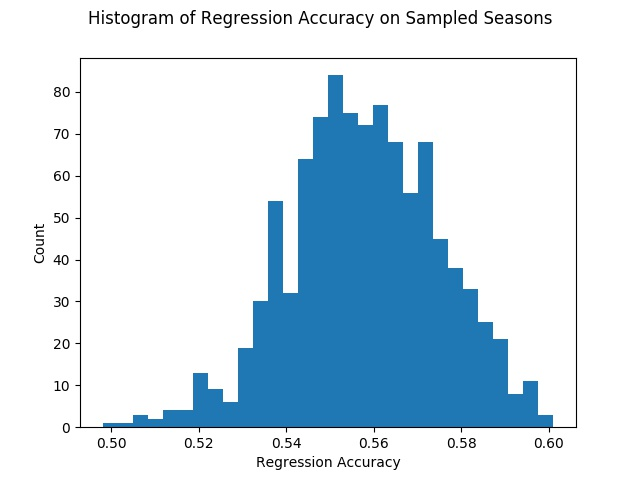
\includegraphics[width=.8\textwidth]{hist_acc.jpg}
    \caption{Figure \label{Fig:SampResults} represents the counts of season
    accuracy for the regressions on the 1000 sampled seasons.}
\end{figure}
The histogram indicates a mostly normal distribution,
perhaps slightly skewed to the left because of the few seasons that had 
accuracies near 50\%.
The best accuracy for a season was just before 60\%,
which is an improvement over the simple win percentage and Pythagorean score
models.
However,
no calculation was made to see if the simple models would have outperformed 
the regression in that particular sample season.

\subsection{Discussion / Future Work}
Logistic regression provided no predictive benefit,
even when combining variables that indicated a baseline tendency for good
prediction.
From the RFR,
the inclusion of weather data was only useful for the first half of the season,
and was only vital for about the first week of the season.
The high correlations among many of the variables in the dataset likely
contributed to the lack of predictive power of the logistic regressor.
More weather categories would likely improve the impact of the weather on the
outcomes of games.
For instance,
finding reliable wind and cloud cover data would likely improve accuracy due
to the real effect those weather patterns have on baseball games. \par

One avenue of increasing prediction accuracy could be using L1 normalization 
on the logistic regression with a very small threshold for feature inclusion.
This would simulate Lasso-Regression for dynamic feature selection as the
season progresses.
This would allow for the inclusion of features to be a dynamic process 
potentially giving greater predictive accuracy. \par

Another potential avenue for increasing prediction accuracy is including more
variables that do not monotonically increase as the season progresses.
Instead of cumulative runs scored and allowed,
perhaps simply using the runs scored and allowed by each team in the previous
game.
For the simulated seasons,
this should drastically reduce the correlations betweens 
runs scored and allowed.
Additionally,
perhaps including the strength of the opponents schedule would help give more
weight to each teams current win percentage entering the game.
There are many exciting possibilities to improve accuracy,
and I am not giving up on this idea just yet.

\newpage
\bibliography{report_bwhitne1}
\bibliographystyle{ieeetr}
\end{document}
